
\section{GraphCoQL}\label{sec:form}

In this section we describe our formalization of GraphQL in Coq. We start by defining a schema and its properties, then the graph data model and finally we review queries and their semantics. The definitions are as close as possible with respect to the \spec{}. This eyeball correspondence between the english-written definitions and the code gives a first level of trust that our formalization is correct, following the examples of X, Y and Z. Whenever there is a mismatch we point it out and explain the reasoning behind each decision.

 \td{mention that we want to correlate to the spec and eyeball correspondence when possible.}

\td{The definitions consist of around 3700 loc and 1400 of lemmas}.

\subsection{GraphQL Schema}\label{subsec:schema}

The GraphQL schema is pretty straightforward to define from the grammar of the \spec{}. It consists of a collection of type definitions and a root query operation type. There is, however, a slight ambiguity when the \spec{} refers to the schema, as it is described as being ``\textit{defined in terms of the types and directives it supports as well as the root operation types for each kind of operation}''\footnote{https://graphql.github.io/graphql-spec/June2018/\#sec-Schema}. It then proceeds to define a structure called \texttt{schema} containing only the root operation types (query, mutation and subscription) and \textit{separately} it defines the type definitions, as well as the directives. The previously quoted definition actually matches the \textit{Type System} structure\footnote{https://graphql.github.io/graphql-spec/June2018/\#TypeSystemDefinition}. Our formalization follows the latter but rename it to schema to also match the quoted description.

\begin{minted}{coq}
Record graphQLSchema := GraphQLSchema {
    query_type : Name;
    type_definitions : seq TypeDefinition
}.
\end{minted}

Similarly, for type definitions we follow the grammar as specified in the \spec{}. Figure \ref{fig:types_def} shows the grammar and the corresponding implementation in Coq. As can be seen from the figure, our implementation looses information about non-emptiness of fields, union and enum members. We push this validation to a posterior predicate, as well as the discussion about the reasons behind this decision, to the following paragraphs.

% As can be seen in the figure, we tried to match the \spec{}'s definition as much as possible. This eyeball correspondence gives us a degree of confidence about the implementation.  % We currently do not include the \textit{Input Object} types, as well as anything related to \textit{introspection}.

Although the definitions are straightforward, both the \spec{}'s grammar and the Coq implementation allow building invalid schemas. For instance, it is possible to build an Object that implements scalar types or use a nonexistent type as the query type. To this end, the \spec{} includes validation rules scattered throughout the document\footnote{Most can be found in the \textbf{Type Validation} subsection of each type described in https://graphql.github.io/graphql-spec/draft/\#sec-Type-System.}. In \coql, we summarize these rules into predicates and refer to it as the \textit{well-formedness} property of a GraphQL schema. \HP{} refers to this property as the \textit{consistency} of the schema, to which we will refer briefly in a following paragraph.


\begin{definition}
A GraphQL schema is \textit{well-formed} if it satisfies the following conditions:
\begin{itemize}
    \item Its root query type is defined and is an Object type.
    \item There are no duplicated type names.
    \item Every type definition is \textit{well-formed}.
\end{itemize}
\end{definition}

The implementation in Coq is described by the following boolean predicate. As indicated in the introduction of this paper, we try to use boolean reflection as much as possible, following the SSReflect mindset.

\begin{minted}{coq}
Definition is_a_wf_schema (s : graphQLSchema) : bool :=
      is_object_type s s.(query_type) &&
      uniq s.(schema_names) &&
      all is_wf_type_def s.(type_definitions).
\end{minted}

Due to space constraints, we omit the definition of well-formedness for type definitions. The complete definitions can be found in the file \texttt{SchemaWellFormedness.v}. We will, though, resume the discussion about non-emptiness of fields, union and enum members, which are included in the predicate. The main reason behind this decision is that, even though the \spec{} embeds this information in the grammar, it still includes it in their validation rules later on. We believe that it is simpler to use common lists instead of defining new structures or using dependent types, from an implementation point of view, while still preserving the correspondence to the algorithmic description given by the \spec{}.
\td{Not sure if correctly worded... but it was just simpler to use lists. A non-empty list structure required coercions to lists and then redefining some lemmas and things. Or using dependent types (sigma type) adds complexity when proving and defining things (at least that was the case for me)}

Regarding \HP{}'s consistency property, they embed many properties in their structures, such as uniqueness of types given by using sets. They include an additional check on objects implementing interfaces, where they validate that fields are properly implemented. The definition given is not complete due to missing validation on arguments, but a corrected version is included in \cite{olafschema}.

% There are two main reasons why we push this rule to a separate predicate instead of embedding it in the structure itself. The first one is that, even though the \spec{} embeds it in the grammar, it still includes it in a validation rule later on. To match their definition and preserve the eyeball correspondence, we also include it. The second reason is that we use SSReflect and it is simpler to use \mintinline{coq}{seq} directly and all its theory, instead of defining coercions and repeating definitions for a new structure.


With the well-formedness property, we proceed to define a structure that encapsulates this notion, by passing both a schema and a proof of its validity.

\begin{minted}{coq}
Record wfGraphQLSchema := WFGraphQLSchema {
    schema : graphQLSchema;
    _ : schema.(is_a_wf_schema);
    is_a_valid_value : type -> Vals -> bool;
}.
\end{minted}

It is immediate that this structure requires an additional \mintinline{coq}{is_a_valid_value} predicate, which receives an element of \texttt{type} and a value of type \texttt{Vals}. This predicate is necessary to establish when a value used in a query or in the graph actually matches the scalar type expected by the schema. For instance, if an argument requires a \texttt{Float} value, then the actual value passed to the query must be something that represents a double-precision fractional value\footnote{The \spec{} declares a set of minimal scalar values and how they should be represented, such as floating-point values adhering to IEEE 754. We do not include this base restrictions but leave it open to implementation.}. This predicate validates that this is satisfied.

% Due to space constraints, we omit the definition of \textit{well-formedness} for type definitions. This property includes things such as: interfaces and objects must declare at least one field, objects correctly implement their declared interfaces, union types are not empty and contain only object types, amongst others. These definitions are collected from the \spec{} \td{Scattered throughout the \spec{}*}.

Finally, having defined the GraphQL schemas, we can move onto defining the data model used when evaluating queries.

\setlength{\grammarparsep}{20pt plus 1pt minus 1pt} % increase separation between rules
\begin{figure*}
    \centering
    \begin{subfigure}{.5\textwidth}
    \begin{grammar}
    <TypeDefinition> ::= \textbf{scalar} <name>
    \alt \textbf{type} <name> \textbf{implements} <name>* \textbf{\{} <Field>+ \textbf{\}}
    \alt \textbf{interface} <name> \textbf{\{} <Field>+ \textbf{\}}
    \alt \textbf{union} <name> \textbf{=} <name> \textbf{|} <name>*
    \alt \textbf{enum} <name> \textbf{\{} <name>+ \textbf{\}}

    <Field> ::= <name> \textbf{(} <Arg>* \textbf{) :} <type>

    <Arg> ::= <name> \textbf{:} <type>

    <type> ::= name
    \alt \textbf{[}  <type> \textbf{]}
    \end{grammar}

    \caption{Grammar of GraphQL types}
    \end{subfigure}%
    \begin{subfigure}{.5\textwidth}
    \begin{minted}{coq}
    Inductive TypeDefinition : Type :=
    | ScalarTypeDefinition (name : Name)

    | ObjectTypeDefinition (name : Name)
                           (interfaces : seq Name)
                           (fields : seq FieldDefinition)

    | InterfaceTypeDefinition (name : Name)
                              (fields : seq FieldDefinition)

    | UnionTypeDefinition (name : Name)
                          (members : seq Name)

    | EnumTypeDefinition (name : Name)
                         (members : seq EnumValue).

    Inductive type : Type :=
    | NamedType : Name -> type
    | ListType : type -> type.
    \end{minted}

    \caption{Implementation in Coq\td{Should include fields and arguments?}}
    \end{subfigure}
    \caption{Definition of GraphQL types.}
    \label{fig:types_def}
\end{figure*}



\iffalse
\begin{minted}{coq}
Let Animal := Interface "Animal" {[::
                (Schema.Field "name" [::] "String");
                (Schema.Field "friends" [::] ["Animal"])
            ]}.
Let Dog := Object "Dog" implements [:: "Animal"] {[::
            (Schema.Field "name" [::] "String");
            (Schema.Field "friends" [::] ["Animal"]);
            (Schema.Field "favouriteToy" [::] "Toy")
        ]}.
\end{minted}
\fi

\subsection{GraphQL Data model}\label{subsec:graph}

GraphQL is not tied to any particular database technology and implementation. When resolving fields in a query, GraphQL assumes the existence of \textit{resolvers}. These are internal functions defined by the user implementing a GraphQL service. They are not tied to any particular data model and the only requirement is that they must adhere to the schema. Whether they access a database, return static values or even modify existing data, is up to the user\footnote{The \spec{} states that these ``\textit{must always be side effect‐free and idempotent}'' but the definition of a resolver does not actually impose these restrictions.}. This makes reasoning about the semantics hard.

We choose to follow \HP{}'s approach and define the underlying data model as a graph over which queries are evaluated. With this model, the unspecified resolvers can be instantiated to concrete definitions which allow reasoning over them. The semantics are then described as being implemented over a graph setting. Although this provides benefits when reasoning about the semantics, it also comes with some potentially severe limitations over the completness of the possible results generated.\td{They may not actually be limitations with the model, but there are open questions on how to model some things.} We cover these limitations more thoroughly in a following paragraph and in Section~\ref{subsec:semantics}. It is worth mentioning that the limitations of this model are not described nor discussed in \HP{}.

Informally, a GraphQL graph is a directed property graph, with labeled edges and typed nodes. The graph describes entities with their types and properties, as well as the relationship between them. This means that every node has properties (key-value pairs) and a type. Also, every label in an edge describes the relation between two nodes. Finally, every property or label may also contain a list of arguments (key-value pairs).

We consider the type \Vals, representing the values associated to properties or used for arguments. A value in \Vals{} may be a single scalar value or a list of values.

\begin{definition}
A GraphQL graph over \Vals is defined by the following elements:
\begin{itemize}
    \item A root node.
    \item A collection of edges of the form ($u$, \texttt{f[}$\alpha$\texttt{]}, $v$), where $u, v$ are nodes and \texttt{f[}$\alpha$\texttt{]} is a label with arguments (key-value pairs).
\end{itemize}
\end{definition}

This is defined with the following structures in Coq.

\begin{minted}{coq}
Record fld := Field {
                  label : string;
                  args : seq (string * Vals)
                }.

Record node := Node {
                   ntype : Name;
                   nprops : seq (fld * Vals)
                 }.

Record graphQLGraph := GraphQLGraph {
                        root : node;
                        E : seq (node * fld * node)
                      }.
\end{minted}

\td{probably rewrite this paragraph...}
Our definition is in essence the same as in \HP{} but differs greatly in implementation. \HP{} defines a GraphQL graph in a more ``centralized'' manner. For instance, nodes and field names are defined by sets. Node types are defined by a single function which receives a node identifier and gives its type. Properties are also defined by a single function which receives a node identifier and a field name with arguments. Contrarily, our approach attempts to recreate the structures individually. For instance, a node contains all the information pertaining to itself; its type and its properties. We believe this is a more natural approach to defining the graph from an engineering point of view.

The definition of graph is completely independent of any GraphQL schema, so we need a way to relate the data to the type system. We implement the notion of \textit{conformance}  of a graph as partially described by \HP{}. This notion is, in essence, a well-formedness property for graphs with respect to a given schema. At the moment of development, there was no complete definition of conformance given by \HP{}. However, in a recent work by Hartig and Hidder's~\cite{olafschema}, they give a complete definition and extend it. Their approach uses a similar ``decentralized'' idea to define graphs. Their definitions capture more features than we currently implement, such as directives and non-null types.\td{And variables if I'm correct - should check}

\begin{definition}
A GraphQL graph \textit{conforms} to a schema $\mathcal{S}$ if it satisfies the following conditions:
\begin{itemize}
    \item The root node's type is equal to the query type.
    \item Every edge \textit{conforms} to $\mathcal{S}$.
    \item Every node \textit{conforms} to $\mathcal{S}$.
\end{itemize}
\end{definition}

This is captured in the following predicate in Coq.
\begin{minted}{coq}
Definition is_a_conforming_graph
        (s : wfGraphQLSchema)
        (graph : graphQLGraph) : bool :=

        root_type_conforms s g.(root) &&
        edges_conform s g &&
        nodes_conform s g.(nodes).
\end{minted}

Similarly to GraphQL schemas, we define a structure that encapsulates the notion of a \textit{conformed} graph. It contains a graph and a proof of its \textit{conformance} to a particular schema.

\begin{minted}{coq}
Record conformedGraph (s : wfGraphQLSchema) :=
            ConformedGraph {
                graph : graphQLGraph;
                _ : is_a_conforming_graph s graph
            }.
\end{minted}

Due to space limitations, we omit a detailed review of \textit{conformance} of nodes and edges. The complete definitions can be found in the file \texttt{GraphConformance.v}. %These properties include validation rules such as: every node must have an object type and their properties must be defined in their associated type, or an edge's label must be declared as a field in the source node's type and the target node must have a type compatible to the field's return type, among other things.

Finally, we partially retake the discussion on the limitations of this model. These have consequences on the semantics of GraphQL queries, so we delay some of it to the corresponding section. The main issue is that there is no proper accounting with respect to list types containing other list types (with any nesting depth). The different features that compose a GraphQL schema can be translated to a graph somehow. For instance, a field is either a property or the label of an edge, while its return type can be associated to a target node in an edge. However, when it comes to list types it is not clear what they represent in a graph. Let us illustrate this with an example.

A service may declare the field \texttt{friends:[Human]} in a given type, representing the list of friends.
In a graph this can be pictured as having a node with multiple outgoing edges labeled \texttt{friends}, reaching other nodes of type \texttt{Human}. It is possible to then extend the service by including a new field \texttt{friendsByName:[[Human]]}, in which one can request a list of friends but grouped by their names. At the moment neither our implementation, \HP{} nor \cite{olafschema} properly handle this situation. The open question is what does this represent in the graph? These should be outgoing edges similarly to the previous case but, what should the target nodes be? Should these be intermediate blank nodes? Is every edge labeled or only the last one that reaches a node with type \texttt{Human}? What happens if we increase the nesting? Since the information is ultimately collected from ``concrete'' nodes, should the graph be kept the same but introduce \textit{formatter} functions to match the schema?

These questions and more are not addressed nor discussed in \HP{} and it is actually more restrictive than expected, by not allowing nested lists for scalar values (in nodes's properties). Meanwhile, our approach and the one used in \cite{olafschema} allow any list type at the property level but simply ignore any possible nesting when the list type refers to neighboring nodes (composite types), as in the example above. In the case of \cite{olafschema}, they do not address nor discuss these questions. This choice of modeling has some consequences when defining the semantics of GraphQL queries, because the possible results generated are restricted to a smaller subset. It is not clear what the proper way is to handle this issue but more is explored in Section~\ref{subsec:semantics}. We also address the \spec{}'s semantics and how this is managed.

With both the schema and the underlying data model we can proceed to define GraphQL queries and their semantics.

\subsection{GraphQL Query}\label{subsec:query}

As we mentioned in section \ref{sec:bg}, GraphQL queries are selections over types and fields defined in the schema. A GraphQL query can be seen as a tree structure where leaf nodes are selections of fields with a scalar return type. An inner node can be a selection on fields with an object or abstract return type. Inline fragments that condition when its subqueries are evaluated can also be seen as inner nodes. For instance, the query in Figure \ref{fig:qres_ex} can be depicted as the tree in Figure \ref{fig:query_tree}.

\begin{figure}
    \centering
    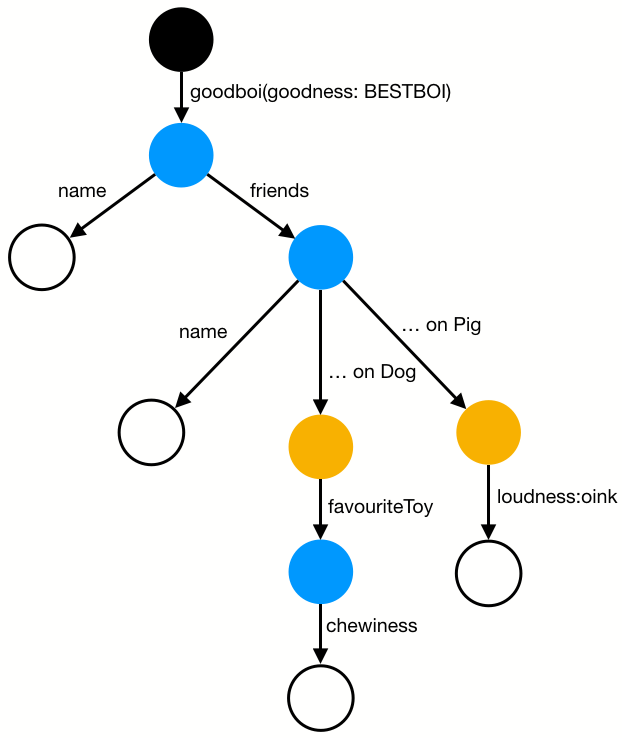
\includegraphics[scale=0.33]{imgs/query_tree.png}
    \caption{GraphQL query as a tree.}
    \label{fig:query_tree}
\end{figure}

Similar to the schema definition, we try to follow the \spec{}'s grammar as closely as possible. The grammar and implementation can be seen in Figure~\ref{fig:query_def}. There is a lost of information regarding non-emptiness of subqueries, as seen by rule 2 and the constructor \texttt{NestedField}. The reasoning behind this decision is very similar to the one used when implementing type definitions, which is described in Section~\ref{subsec:schema}.

\begin{figure*}
  \centering
  \begin{subfigure}{.5\textwidth}
    \begin{grammar}
        <Query> ::= <name> \textbf{(} <Arg>* \textbf{)}
        \alt <alias> \textbf{:} <name> \textbf{(} <Arg>* \textbf{)}
        \alt <name> \textbf{(} <Arg>* \textbf{)} \textbf{\{} <Query>+ \textbf{\}}
        \alt <alias> \textbf{:} <name> \textbf{(} <Arg>* \textbf{)} \textbf{\{} <Query>+ \textbf{\}}
        \alt \textbf{... on} <name> \textbf{\{} <Query>+ \textbf{\}}

        <Arg> ::= <name> \textbf{:} <value>
    \end{grammar}
    \caption{Grammar of GraphQL queries}
  \end{subfigure}%
  \begin{subfigure}{.5\textwidth}

    \begin{minted}{coq}
    Inductive Query : Type :=
    | SingleField (name : Name)
                  (arguments : seq (Name * Vals))

    | AliasedField (alias : Name)
                   (name : Name)
                   (arguments : seq (Name * Vals))

    | NestedField (name : Name)
                  (arguments : seq (Name * Vals))
                  (subqueries : seq Query)

    | NestedAliasedField (alias : Name)
                         (name : Name)
                         (arguments : seq (Name * Vals))
                         (subqueries : seq Query)

    | InlineFragment (type_condition : Name)
                     (subqueries : seq Query).
    \end{minted}
    \caption{Implementation in Coq}
  \end{subfigure}
  \caption{Definition of GraphQL queries.}
  \label{fig:query_def}
\end{figure*}


Both the \spec{} and our formalization differ from \HP{} when defining queries. The main difference is that \HP{} include an additional rule for lists of queries. Their grammar includes a production rule for lists of queries which is at the same level of the other rules. The main issue we found with this approach is that it allows building arbitrary trees instead of just a list of queries. These trees can be flattened to recover the list structure but this represents additional effort when defining functions and reasoning over queries. We believe this is assumed by \HP{} but not explicitly mentioned otherwise.


As in the case of well-formedness of schemas or conformance of graphs, queries must go through a validation process. We define the \textit{conformance} of queries based on validation rules scattered throughout the \textit{Validation} section of the \spec{}\footnote{https://graphql.github.io/graphql-spec/June2018/\#sec-Validation}.

Before defining the validation process, it is very important to address the notion of \textit{type in context} where selections are used. This notion is necessary to validate queries and when transforming queries, as described in Section~\ref{sec:norm}. The type in context is the type over which someone might be requesting information on its fields. For instance, in the following example the field selection \texttt{goodboi} is used in the context of the \texttt{Query} type. However, the type in the case of the field \texttt{name} is not entirely clear. In one case, the type in context is \texttt{Dog}, while in the other the field is used in the context of the \texttt{Pig} type.

\begin{minted}[escapeinside=||, mathescape=true]{js}
      query {
        goodboi {
          |$\ldots$| on Dog {
            name
          }
          |$\ldots$| on Pig {
            name
          }
        }
      }
\end{minted}

The importance of this type in context is that fields or inline fragments might be valid in certain cases but not in others. Similarly, a field may have a particular return type in one case and a different one in another type, like in the following example. Both types have an \texttt{age} field, but in one case it returns an integer value while in the other a floating point value. If that field is encountered in a query, it is necessary to know to which type it is being requested.

\begin{minted}{js}
      type Human {
        age: Int
      }

      type Martian {
        age: Float
      }
\end{minted}


\begin{definition}
A GraphQL query $\varphi$ \textit{conforms} to a schema $\mathcal{S}$ if it satisfies the following conditions:
\begin{itemize}
    \item Selections in $\varphi$ are consistent.

    \item Field merging between fields is possible.
    % During the evaluation process, fields with the same response name are collected and merged to ensure that they are all executed at the same time. This validation rule checks that it makes sense to merge those fields. The following example illustrates two queries that have the same response name but should not be merged. The first one is accessing the field \texttt{name} while the second is accessing the field \texttt{age} but renaming it to \texttt{name}. Both are selections on different fields of the same type but with the same response name.
    % \begin{minted}{graphql}
    %                query {
    %                    name
    %                    name:age
    %                }
    %\end{minted}

    \item Fields with same response name have compatible response shapes.
    % This checks whether two fields with the same response name will produce response values that are consistent to each other. These values should be unambiguous for a user. For instance, the following example\td{These examples look a bit off I think.} shows two queries that produce similar responses but with ambiguous values. In the first one, we ask for dog's \texttt{name}s, which are strings, and in the second for pig's \texttt{age}s, which are integers. We also rename the \texttt{age} value to \texttt{name}. The responses we get will have some cases where \texttt{name} is associated to a string and other where it is associated to integers.
    % \begin{minted}[escapeinside=||,mathescape=true]{graphql}
    %                query {
    %                    |$\ldots$| on Dog {
    %                        name
    %                    }
    %                    |$\ldots$| on Pig {
    %                        name:age
    %                    }
    %                }
    % \end{minted}
\end{itemize}
\end{definition}

The definition in \coql{} is given by the following code. Due to space constraints, we do not include the complete definitions but they can be found in the file \texttt{QueryConformance.v}.

\begin{minted}{coq}
Definition queries_conform (type_in_scope : Name)
                           (queries : seq Query) : bool :=
        all (is_consistent type_in_scope) queries &&
        is_field_merging_possible type_in_scope queries &&
        have_compatible_response_shapes
            [seq (type_in_scope, q) | q <- queries].
\end{minted}

As described earlier, this rules are mostly a condensation of a set of validation rules defined in the \spec{}. The first one refers to whether a selection holds by itself. It includes checks such as: if query is over a field, then that field must be defined in the  type in context and its arguments are defined in the given field. Similarly, if a selection is an inline fragment, then the type condition has to be valid with respect to the type in context.

The second and third predicates are defined as a single validation rule in the \spec{}\footnote{https://graphql.github.io/graphql-spec/June2018/\#sec-Field-Selection-Merging}. We split them into two separate predicates because there is a chance for optimization. We noticed that the original definition includes redundant recursive calls which may result in increased computational time. At the time of writing this paper, a new algorithm was proposed by a team at XING\footnote{https://www.xing.com/} that also addresses this very same issue and is described in~\cite{xingalg}. They follow an approach using sets and provide a much more elaborate analysis of execution times than us. Comparing both approaches and analyzing execution times could be an interesting venue to explore.

During development, we also noticed that the \spec{}'s rule is too conservative and may consider valid queries as invalid. In a nutshell, the \spec{} allows defining fragments that are never evaluated. The issue is that the validation rule can then consider that subqueries in these fragments are invalid, even though they are never evaluated, rendering the whole query invalid\footnote{An example query can be seen in the following link: https://tinyurl.com/y3hz5vgv.}. The definition of the second predicate attempts to remove this conservativeness but we have not proved it. For the third predicate, we still have some conservative checks. Section \ref{subsec:invalidfrags} delves a little deeper into this issue.

% The main issue is that the \spec{} allows for what we call \textit{invalid fragments}, originally described in an issue in the \spec{}'s repository\footnote{https://github.com/graphql/graphql-spec/issues/367}. In a nutshell, the \spec{} allows using fragments with type conditions that can span to multiple unrelated types. These end up not being evaluated due to posterior checks\footnote{https://graphql.github.io/graphql-spec/June2018/\#DoesFragmentTypeApply()}.


Finally, with these definitions we can build queries in a GraphQL service. Examples may be found in the files \texttt{SpecExamples.v} and \texttt{HPExample.v}. From now on, we will assume that queries conform to a given schema. We can then move onto their semantics.

\subsection{Semantics}\label{subsec:semantics}

In this section we describe the semantics of GraphQL queries. We begin by briefly examining the responses generated by executing queries. Then we give an informal description of the semantics, followed by the formal definition. We finish by discussing some implementation choices and comparison with the \spec{} and \HP{}.

The \spec{} describes responses as a map. Our implementation differs slightly, modeling them as a tree structure, similar to JSON. We choose this structure to preserve similarity to queries and because it is simpler to preserve order of the responses. The \spec{} does not impose an ordering of responses, although encourages it\footnote{https://graphql.github.io/graphql-spec/June2018/\#sec-Serialized-Map-Ordering}. We believe that preserving the order is one of the selling points for GraphQL (queries and their responses are very similar and easy to read). Our approach has two main disadvantages: uniqueness of response names and cost of access. Since we use lists instead of maps, we can encounter duplicated names and accessing a value has a linear cost given by the lists size, instead of the constant access obtainable with a map. We still argue that the simplicity to obtain order is worth it. We do include a proof that the results obtained with the semantics have unique names. Finally, we use option types to represent null values in the leaves of the response tree.

\begin{minted}{coq}
Inductive ResponseNode (A : Type) : Type :=
| Leaf : A -> ResponseNode
| Object : seq (Name * ResponseNode) -> ResponseNode
| Array : seq ResponseNode -> ResponseNode.

Definition GraphQLResponse (Vals: eqType) :=
    seq (Name * (@ResponseNode (option Vals))).
\end{minted}

Moving onto the semantics of GraphQL queries. As we described in Section~\ref{subsec:graph}, the underlying data model is a graph, therefore the semantics are instantiated to this setting. In a following paragraph we briefly explore an alternative that is closer to the \spec{}, in the sense that it can be detached from a particular data model. In our setting a query then represents a navigation over a graph. At top level, a query starts from the root node and then moves around its edges and nodes, collecting data along the way. In this sense:
\begin{itemize}
    \item A field selection represents either accessing a node's property or traversing an edge to a neighboring node. On the neighboring nodes we recursively evaluate subqueries.
    \item An inline fragment conditions whether using a node to access its properties or to traverse to other nodes.
\end{itemize}

Figure \ref{fig:semantics} shows the formal definition of the semantics. It displays the cases where a field selection is accessing a node's property, when it is navigating to other nodes and when it is evaluating an inline fragment. Aliased fields are omitted for brevity but the complete definition can be explored in the file \texttt{QuerySemantics.v}.

The main difference with respect to \HP{} and the main similarity to the \spec{} is that we perform a collection of fields at the query level, whereas \HP{} performs a post-processing of responses. The main reasons are similarity to the \spec{} and difficulty in reasoning with \HP{}'s approach, which we explore in more depth in Section~\ref{subsec:semstories}.

%Our first attempt at defining the semantics was to follow \HP{}'s post-processing approach. Our intention was to be as close as possible to their formalization to later prove their transformation and equivalence results, which we cover in Section~\ref{sec:norm}. However, the non-structural recursive nature of both the transformations and the post-processing function made reasoning about semantic equivalence very hard.

\begin{figure*}
    \centering
    \begin{align}
    % Empty
    \eval{\cdot}{u} &= [\cdot] \\
    % SingleField
    \evalu{\fld\; ::\; \queries} &= \begin{cases}
    \resp{\val} \; ::\; \evalfilteru{\queries}{\fkey}  & \mathit{u.property}(\fld) = \val \\
    \resp{\nval} \; :: \; \evalfilteru{\queries}{\fkey} & \sim
    \end{cases}\\
    % Nested field
    \evalu{\nfld{\overline{\beta}} \; ::\; \queries} &=
    \begin{cases}
    \resp{\texttt{[} \mathit{map} (\lambda\; v_{i} \Rightarrow \eval{\overline{\beta} \mdoubleplus \mathit{merge (collect_\fkey (\queries))}}{v_{i}})\; \mathit{neighbors(u)} \texttt{]}} \; :: \; \evalfilteru{\queries}{f}  & \mathit{type(f)} \in L_{t} \text{and} \{v_{1}, \ldots, v_{k}\} = \{v_{i} \mid (u, f[\alpha], v_{i}) \in E\} \\
    (f:\{\eval{\subqueries{\beta}}{v}\})\; :: \; \evalfilteru{\queries}{f}  & \mathit{type(f)} \notin L_{t} \text{and} (u, f[\alpha], v) \in E \\
    (f:null)\; :: \; \evalfilteru{\queries}{f} & \mathit{type(f)} \notin L_{t} \text{and there is no } v \text{ s.t.} (u, f[\alpha], v) \in E \\
    \end{cases}\\
    %inline fragment
    \evalu{\ifrag{t}{\overline{\beta}}\; ::\; \queries} &= \begin{cases}
    \evalu{\overline{\beta} \mdoubleplus \queries} & \mathit{does\_fragment\_type\_apply_{\texttt{t}}(u.type)} = \texttt{true}\\
    \evalu{\queries} & \sim
    \end{cases}
    \end{align}
    \caption{Semantics for GraphQL queries.\td{This looks bad but I don't know how to format it :/}}
    \label{fig:semantics}
\end{figure*}

We finish this section by addressing two major aspects about our formalization; completeness and errors.

The first one was briefly mentioned in Section~\ref{subsec:graph}, when discussing the limitations and open questions regarding the graph model. These translate in the fact that we currently do not produce list results with nested lists of objects. For instance, the field \texttt{friendsByName:[[Human]]} is treated as if it were defined as \texttt{friendsByName:[Human]} and the results match the latter format. Otherwise, there is no restriction in the case of nested lists for scalar values. In \HP{}, there is no possibility to produce nested lists for either scalar or object values\footnote{The grammar itself does not permit it.} and there is no mention of this restriction.

Regarding error handling, we currently do not implement it. Errors may have two main sources; validation errors and execution errors.\td{Not sure how to write this}

%The first one is that we currently do not handle errors during execution. This is due to two main reasons: the evaluation function assumes it receives valid queries and we have not yet implemented non-null types. These relates to the two kinds of errors one may encounter when evaluating GraphQL queries: validation and execution errors. The first ones are captured before execution and displayed to the user. Our semantics has to deal with a case which would be ruled out by the validation process. We believe both cases can be covered by including X (monad/reasonably exceptional type theory/etc)\td{rewrite}.

% The second major aspect refers to completeness. Both our formalization and \HP{}'s do not generate all possible results expected by a GraphQL service. In particular, there is a limitation when generating lists with a nesting bigger than one. it does not generate results for list types of depth bigger than one, when its inner type is not a scalar type\footnote{HP goes a step further and does not allow any type of nested list result.}. For instance, one might want to get information about friends but grouped by their age. This could be modeled as a field with type \texttt{[[Human]]}, where the list type has depth 2. A response for this query would look something like \texttt{"friends":[[...], ..., [...]]}. This response cannot be generated by our semantics\footnote{It can be defined with the \mintinline{coq}{Response} structure but not generated with the semantics.}.

%The main challenge in this case is to define what this nested list types represent in a graph. If we take a simple case of a field with type \texttt{[Human]}, we can model it as neighbors of a node. However, if we increase the nesting such as \texttt{[[Human]]}, it becomes harder to model. What does this represent in the graph? Should we introduce blank nodes in between the source node and the \texttt{Human} nodes? Are these inner edges labeled? Should there be a blank node per each level of nesting or a single one with edges to itself? All these questions do not have a straightforward answer. Our semantics, as the one definded in PH, simply ignores any nesting bigger than one.\td{This is where it can be modelled using Functors. The \spec{} checks if it received a collection and applies map to eventually get to the concrete values. Not sure how to put this out there.}
\td{I am also missing functors and how the spec "should" be defined.}

This concludes the base formalization of GraphQL schemas, graph data model, and queries and their semantics. Using this basic structures we can start defining query transformations and prove some properties about them.
